\input{sty/pre}

\title{Bachelorarbeit \\ Surface Caching und Lightmapping}
\author{Markus Pawellek}
% \date{}
\newcommand{\email}{markuspawellek@gmail.com}


\begin{document}

	\articletitle

	\begin{figure}[h]
		\begin{subfigure}[b]{0.5\textwidth}
			\center
			\includegraphics{gg_fig/scheme_normal-function_1.pdf}
			% \caption{Verlauf}
		\end{subfigure}
		\begin{subfigure}[b]{0.5\textwidth}
			\center
			\includegraphics{gg_fig/scheme_normal-function_2.pdf}
			% \caption{approximierte Fläche}
		\end{subfigure}
		\caption{Die erste Skizze auf der linken Seite zeigt den Verlauf einer Vertex-Normalen-Funktion $\nu$ anhand eines Beispiels. $A_\triangle$ und $B_\triangle$ sind dabei die Eckpunkte eines Dreiecks $\triangle$. $\mu_A$ und $\mu_B$ sind die jeweilig gegebenen Vertex-Normalen an den Eckpunkten. Im rechten Bereich der Abbildung ist die durch $\nu$ approximierte gekrümmte Fläche $\tilde{S}(\triangle)$, für die Normalen $\nu(x)$ äußere Normalen bezeichnet, eingezeichnet.}
	\end{figure}


	\begin{figure}[h]
		\center
		\includegraphics{gg_fig/triangle_mesh_1.pdf}
		\caption{Die Abbildung zeigt eine beispielhafte Menge von Dreiecken $\set[i\in\SN,i\leq 7]{\triangle^{(i)}}$. Verschiedene Gruppen von Dreiecken bilden eine Approximation einer Oberfläche im Raum. Dabei werden die Eckpunkte der Dreiecke geteilt und es gilt zum Beispiel $\triangle^{(1)}_B=\triangle^{(3)}_A$ und $\triangle^{(1)}_C = \triangle^{(3)}_C$.}
	\end{figure}


	\begin{figure}[h]
		\center
		\includegraphics{gg_fig/ray_tracing_1.pdf}
		\caption{Die Abbildung zeigt eine Skizze, welche das Sichtbarkeitsproblem und den Raytracing-Algorithmus verdeutlicht. Der ausgesendete Strahl trifft in der Szene genau zwei Punkte. Dabei wird der Zweite durch den ersten verdeckt. Für den ersten Punkt ergibt die Sichtbarkeitsfunktion also 1 und für den Zweiten gerade 0.}
	\end{figure}

	\begin{figure}[h]
		\center
		\includegraphics{gg_fig/ray_tracing_2.pdf}
		\caption{}
	\end{figure}

	\begin{figure}[h]
		\center
		\includegraphics{gg_fig/radiance_1.pdf}
		\caption{}
	\end{figure}

	\begin{figure}[h]
		\center
		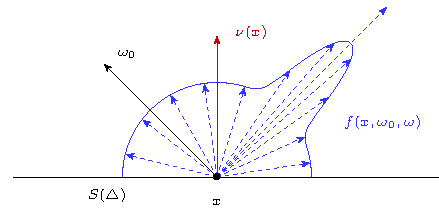
\includegraphics{gg_fig/brdf_1.pdf}
		\caption{}
	\end{figure}


\end{document}